% \documentclass[a4paper,11pt]{article}
% \usepackage[hyperref]{beamerarticle}

\documentclass[final]{beamer}

\usepackage[hangul]{kotex}
\usepackage{amsfonts,amsmath,xob-amssymb}

\usepackage{amsthm}
\newtheorem{defn}{Definition}
\newtheorem{thm}{Theorem}

\usepackage{cancel}
\graphicspath{{./_img/01/}}

\usepackage{graphicx}
\usepackage{media9}

\mode<presentation>{
	\usetheme{Madrid}
	\usecolortheme{default}
	\usefonttheme{professionalfonts}
}

\def\b{\boldsymbol}

\mode<article>{
\usepackage{fullpage}
}
\usepackage{ulem}

\newcommand{\bb}{\mathbb}
\newcommand{\bd}{\mathbf}
\newcommand{\p}{\partial}

\newcommand{\mail}{\url{mailto:experiment.namun+2016f@gmail.com} }


\title{왜 협력인가?}
\subtitle{게임이론이 발견한 놀라운 협력의 비밀들}
\author[조남운]{허준석$\rightarrow$이동한$\rightarrow$\emph{조남운}\\\mail}

\begin{document}

\begin{frame}[t]{}
	\titlepage
\end{frame}
%--- Next Frame ---%

\begin{frame}[t]{목차}
	\tableofcontents
\end{frame}
%--- Next Frame ---%
\section{강사 소개} % (fold)
\label{sec:강사소개}

\begin{frame}[t]{강사 소개 (허준석)}
	\begin{columns}[c]
		\column{16em}
		\begin{itemize}
			\item 경제학 박사 + 30년 넘은 게이머 
			\item (Evolutionary) Game theory vs. Game
			\item 초협력자(사이언스 북스, 2012) 번역 
			\item 재미의 비즈니스(책세상, 2006) 저서
		\end{itemize}
		\column{14em}
		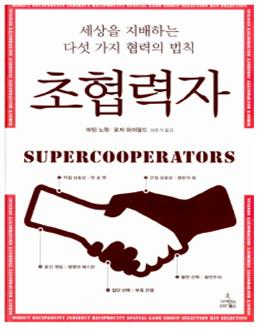
\includegraphics[width=12em]{sck.jpg}
	\end{columns}
\end{frame}
%--- Next Frame ---%

\begin{frame}[t]{강사 소개 (이동한)}
	\begin{columns}[c]
		\column{16em}
		\begin{itemize}
			\item 약사 + 경제학 박사
			\item 관심주제: 참여적 기업시스템
			\begin{itemize}
				\item 성공적인 미국의 노동자 소유 기업을 진화적 게임이론으로 분석 
				\item 소유, 문화, 경영방침 
			\end{itemize}
			\item 에퀴티(지식공작소, 2007) 번역
			\item 노동자가 원하는 것(후마니타스, 2015?) 번역
		\end{itemize}
		\column{14em}
		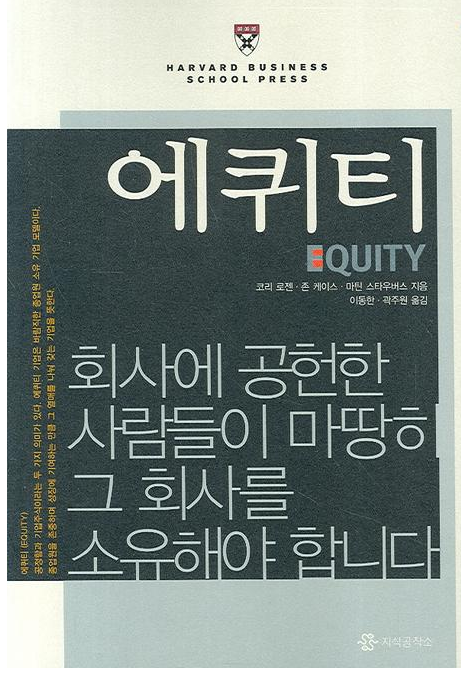
\includegraphics[width=12em]{equity1.png}
	\end{columns}
\end{frame}
%--- Next Frame ---%

\begin{frame}[t]{강사 소개 (조남운)}
	\begin{columns}
		[c]
		\column{.6\textwidth}
		\begin{itemize}
			\item 주관심분야: 진화게임, 행동경제학(실험경제학), 계산경제학 
			\item 경제학 박사
			\item 사적 관심: 자전거타기, 게임, 프로그래밍, 고양이키우기, 키보드
			\item 최근 작업
			\begin{itemize}
				\item 예측시장 (prediction market) 개발, 운영, 분석
				\item 컴퓨터를 사용한 각종 실험들 
			\end{itemize}
			\item \url{http://github.com/z0nam/namun_cho_cv/namun_cv.pdf}
		\end{itemize}
		\column{.4\textwidth}
		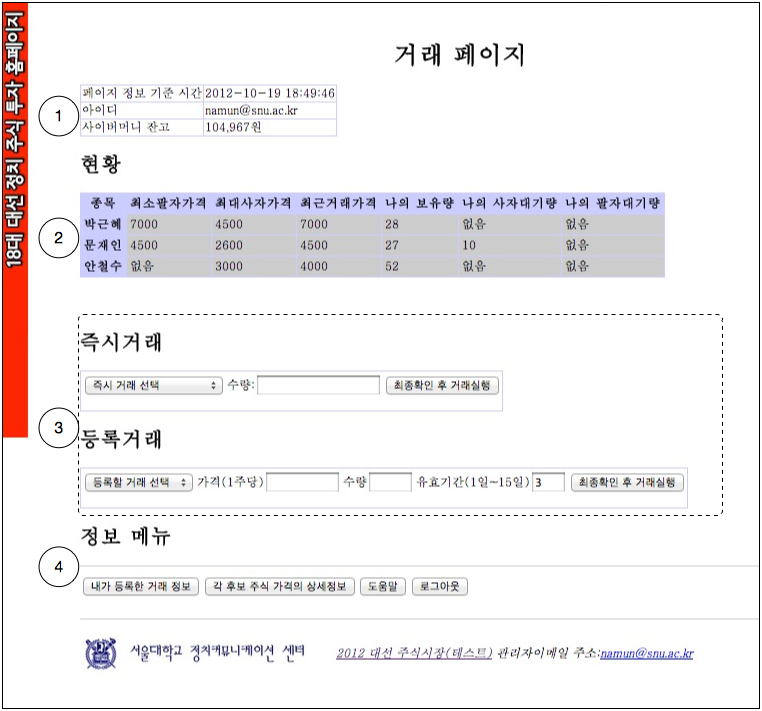
\includegraphics[width=\textwidth]{spsm.png}
	\end{columns}
\end{frame}
%--- Next Frame ---%

% section 강사소개 (end)

\section{경제시스템, 나, 그리고 관계} % (fold)
\label{sec:econSystem}

\begin{frame}[t]{간단한 경제시스템: Sugarscape I}
	\begin{columns}[c]
	\column{16em}
	\begin{itemize}
		\item Joshua Epstein and Robert Axtell (1997)
		\item 원시적인 경제시스템: 출발점
		\item 컴퓨터 모의 실험 (시뮬레이션) 경제적 시스템을 구성
		\item 슈거스케이프(설탕 섬): 물리적 공간, 설탕이라는 에너지원, 차별적인 땅
	\end{itemize}
	\column{12em}
	\fbox{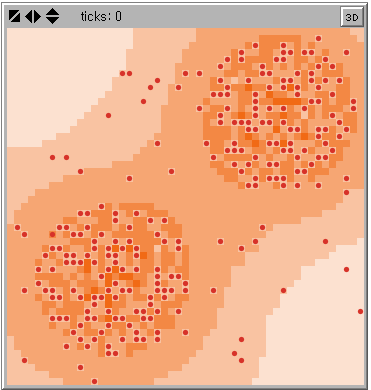
\includegraphics[width=13em]{Sugarscape.png}}
	\end{columns}
\end{frame}
%--- Next Frame ---%

\begin{frame}[t]{Sugarscape I}
	\begin{itemize}
		\item 다수의 Agents(행위자)가 램덤하게 자리를 잡고 출발
		\item Agents(행위자)는 설탕을 찾아 움직이며 설탕을 먹는다
		\item 동서남북 네 방향으로 시각의 범위 내에서 설탕이 많은 비점유 지역을 찾아 이동
		\item 설탕을 획득, 물질대사량 만큼 소비
		\item 획득량 + 저장량 - 대사량 >= 0 $\rightarrow$ 생존, 저장 
		\item 획득량 + 저장량 - 대사량 < 0 $\rightarrow$ 사망 
	\end{itemize}
\end{frame}
%--- Next Frame ---%

\begin{frame}[t]{Sugarscape III}
	\begin{columns}[c]
	\column{17em}
	\begin{itemize}
		\item 설탕이 많이 나오는 땅을 얻기 위한 게임(Hawk-Dove Game)
		\item 혼란 $\rightarrow$ 질서
		\item 시간의 변화에 따른 부의 분포? 80-20 규칙
		\item 불평등한 부의 원인은... 
		\\ $\rightarrow$ 유전자(본성), 태어난 곳(환경), 노력(양육)? 
		\\ $\rightarrow$ No !!!  “모든 것”
	\end{itemize}
	\column{12em}
	%\fbox{
	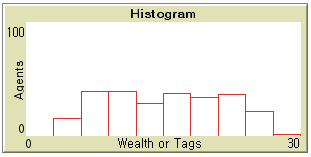
\includegraphics[width=11em]{wealth_histogram01.png} 
	\vspace{3em}
	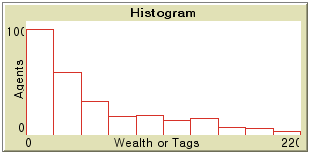
\includegraphics[width=11em]{wealth_histogram02.png}
	%}
	\end{columns}
\end{frame}
%--- Next Frame ---%

\begin{frame}[t]{Sugarscape IV}
	\begin{columns}[c]
	\column{16em}
	\begin{itemize}
		\item 새로운 생산물이 추가: spice(향료)
		\item 설탕, 향료 모두 대사량 보다 적으면 사망
		\item 설탕을 구한 뒤 향료를 구하려 다녀야 함
		\item 거래가 존재한다면? \\
		$\rightarrow$ 거래가 없을 경우 보다 사회의 부가 증가 
	\end{itemize}
	\column{12em}
	\fbox{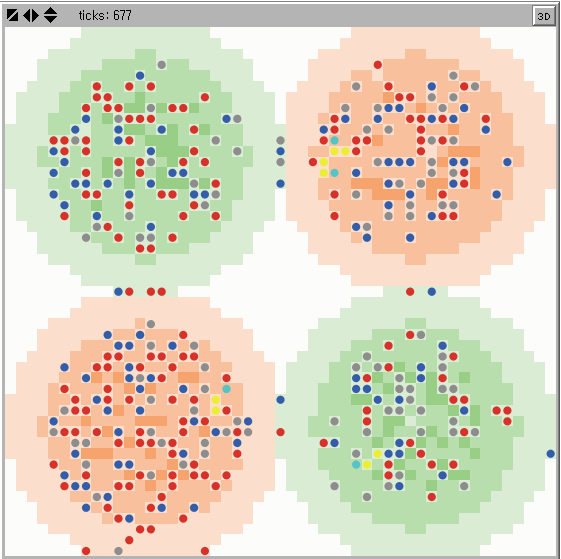
\includegraphics[width=13em]{sugarspice01.png}}
	\end{columns}
\end{frame}
%--- Next Frame ---%

\begin{frame}[t]{불완전 경제 시스템: ACE Trading World}
	\begin{columns}[c]
	\column{18em}
	\begin{itemize}
		\item Tesfatsion and Judd (2005)
		\item 보다 현실적인 경제 모델로 발전
		\item 두 개의 상품을 생산 및 소비하는 다수의 기업, 다수의 생산/소비자가 등장
		\item 합리적인 소비를 하는 소비자, 기업
		\item 균형이 만들어지지만 불완전한 경제시스템
	\end{itemize}
	\column{12em}
	\fbox{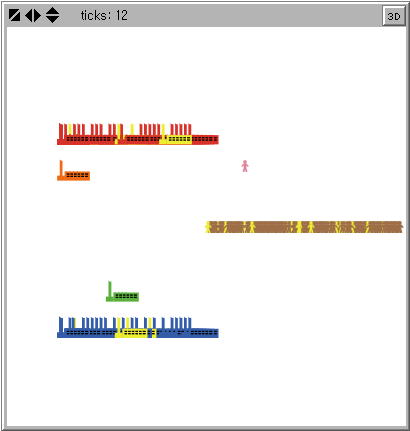
\includegraphics[width=11em]{ACE_TW.png}}
	\end{columns}
\end{frame}
%--- Next Frame ---%

\begin{frame}[t]{자본주의 경제시스템: ACE Capitalist World}
	\begin{columns}[c]
	\column{18em}
	\begin{itemize}
		\item Lee, Dong-Han (2013)
		\item 다양한 게임들로 이뤄진 자본주의 경제시스템
		\item 생산과정에서의 노사 간 협상 게임
		\item 상품시장에서의 기업 간 경쟁 게임 
		\item 노동시장에서의 임금 결정을 둘러싼 게임
		\item 다양한 종류의 관계(게임)로 이루어진 세상 
	\end{itemize}
	\column{12em}
	\fbox{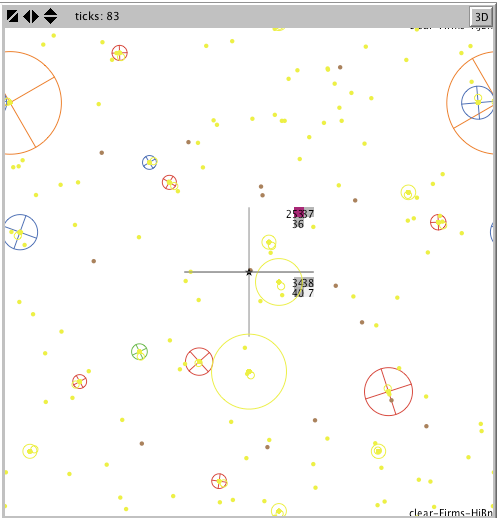
\includegraphics[width=11em]{ACE_CE.png}}
	\end{columns}
\end{frame}
%--- Next Frame ---%

% \begin{frame}[c]{전체 구조}
% 	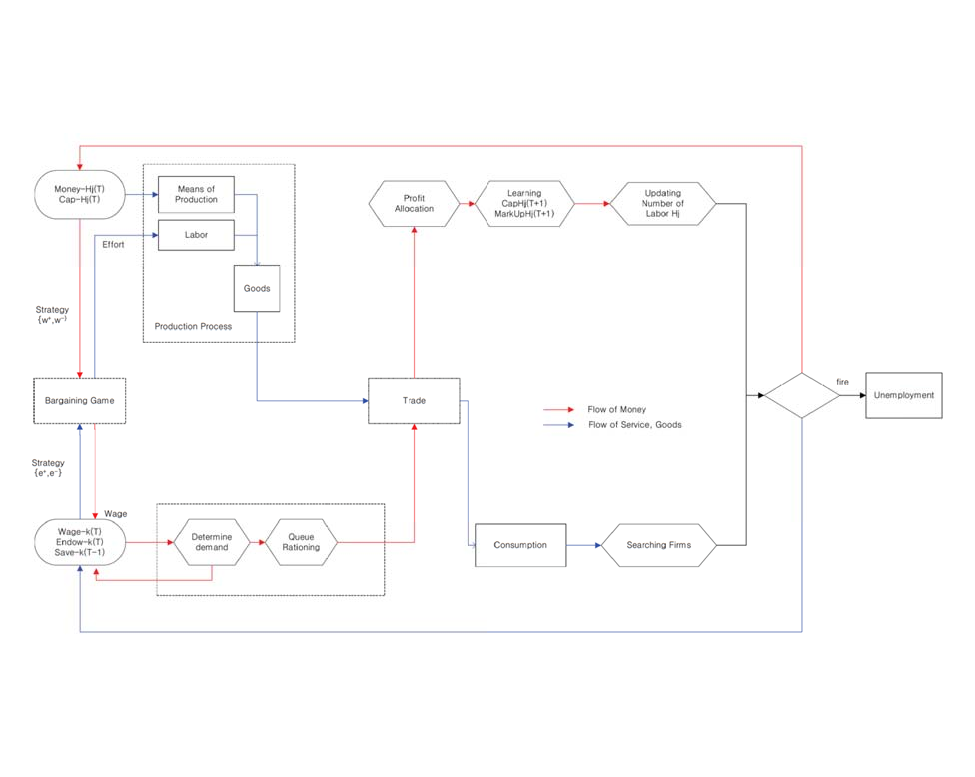
\includegraphics[height=\textheight]{Diag_ACECW.pdf}
% \end{frame}
%--- Next Frame ---%

\begin{frame}[t]{경제시스템, 나, 그리고 게임이론}
	\begin{itemize}
		\item 이 모든 과정들의 변화와 그 과정에서 변화하는 게임들을 수행
		\item 게임 이론은 행위주체들 사이의 다양한 관계를 분석하는 수학적 방법 
		\item 두 사람이 각각 두 가지 전략을 사용하는 서로 다른 게임의 수는 144개
		\item 한 사회를 구성하는 사람들의 관계들을 다양한 종류의 게임들로 분석할 수 있음
	\end{itemize}
\end{frame}
%--- Next Frame ---%

\begin{frame}[t]{2인 2전략 게임의 모든 조합}
	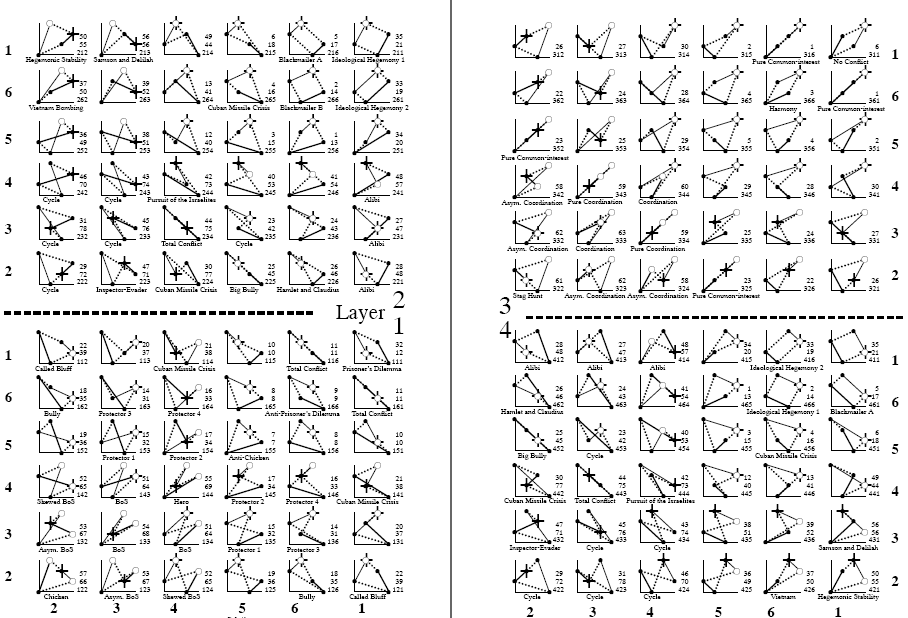
\includegraphics[width=\textwidth]{periodicgametable.png}
\end{frame}
%--- Next Frame ---%

% section econSystem (end)

\section{죄수의 딜레마} % (fold)
\label{sec:PDGame}

\begin{frame}[t]{죄수의 딜레마 (Prisoner's Dilemma)}
	\begin{columns}[c]
	\column{18em}
	\begin{itemize}
		\item 원래 수학적인 정식화는 Merrill Flood와 Melvin Dresher (1950)
		\item 현재의 이야기대로는 Albert W. Tucker (1951)
	\end{itemize}
	\column{12em}
	\fbox{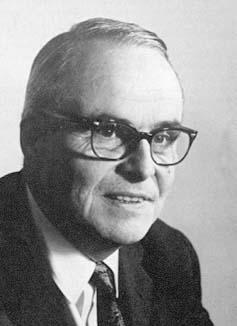
\includegraphics[width=11em]{tucker.jpg}}
	\end{columns}
\end{frame}
%--- Next Frame ---%

\begin{frame}[t]{딜레마 분석하기 - 게임이론의 구성요소}
	\begin{enumerate}
		\item 행위자 (Player)
		\item 결정 (Action/Strategy)
		\item 결과 (Outcome)
		\item 이득 / 손해 (Benefit / Cost, or Payoff)
	\end{enumerate}
\end{frame}
%--- Next Frame ---%

\begin{frame}[t]{죄수의 딜레마의 구성요소}
	\begin{enumerate}
		\item 행위자 (Player) - 2명의 죄수
		\item 결정 (Action/Strategy) - 범행 인정 (C)) / 범행 부인 (D)
		\[
			S = \{C,D\}
		\]
		\item 결과 (Outcome) - 총 4가지의 결과가 존재 가능
		\[
			(S_1, S_2) = \{(C,C),(C,D),(D,C),(D,D)\}
		\]
		\item 이득 / 손해 (Benefit / Cost, or Payoff): 보수행렬 (Payoff Matrix) -- 곧 설명함
	\end{enumerate}
\end{frame}
%--- Next Frame ---%

\begin{frame}[t]{딜레마 분석하기}
	\begin{itemize}
		\item 내가 당할 수 있는 처지도 모두 네 가지 
		\begin{enumerate}
			\item \color{red}{R}\color{black}{eward}
			\item \color{red}{S}\color{black}{ucker}
			\item \color{red}{T}\color{black}{emptation}
			\item \color{red}{P}\color{black}{unishment}
		\end{enumerate}	
		\item 딜레마가 되려면 보수의 크기가 어떻게 되어야 할까? 
	\end{itemize}
\end{frame}
%--- Next Frame ---%

\begin{frame}[t]{보수행렬 (Payoff Matrix)}
	\begin{center}
		\hspace{-6em}
		\begin{tabular}{ccccc}
			%&&\multicolumn{2}{c}{Payoff Matrix}\\
			&&\multicolumn{2}{c}{죄수 2}\\
			&&부인&인정\\
			\cline{3-4}
			\raisebox{-0.25cm}{\rotatebox{90}{1}}&\multicolumn{1}{p{1cm}}{부인}&
			\multicolumn{1}{|p{1.5cm}}{\hfill $-2$\newline $-2$\hfill}&
			\multicolumn{1}{|p{1.5cm}|}{\hfill $-1$\newline $-4$\hfill}\\
			\cline{3-4}
			\raisebox{-0.25cm}{\rotatebox{90}{죄수}}&\multicolumn{1}{p{1cm}}{인정}&
			\multicolumn{1}{|p{1.5cm}}{\hfill $-4$\newline $-1$\hfill}&
			\multicolumn{1}{|p{1.5cm}|}{\hfill $-3$\newline $-3$\hfill}\\\cline{3-4}
		\end{tabular}
	\end{center}
\end{frame}
%--- Next Frame ---%

\begin{frame}[t]{보수행렬 분석}
	\begin{itemize}
		\item 부인 = 협력 (Cooperate), 자백 = 배신 (Defect)
		\item 보수가 마이너스면 보기에 불편하다! 
		\item 모든 값에 $+5$씩 해준다. (이렇게 해도 괜찮을까?)
	\end{itemize}
	\vspace{1em}
	\begin{columns}[c]
		\column{15em}
		\begin{center}
			\begin{table}
				\begin{tabular}{|c|c|c|} \hline
					& {C} &  {D}\\ \hline
					{C} & {-2 + \color{red}{5}}, {-2 + \color{red}{5}} & {-4 + \color{red}{5}}, {-1 + \color{red}{5}} \\ \hline%
					{D} & {-1 + \color{red}{5}}, {-4 + \color{red}{5}}  & {-3 + \color{red}{5}}, {-3 + \color{red}{5}} \\ 
					\hline
				\end{tabular}
			\end{table}
		\end{center}
		\column{15em}
		\begin{center}
			\pause\begin{table}
				\begin{tabular}{|c|c|c|} \hline
					& {C} &  {D}\\ \hline
					{C} & {3}, {3} & {1}, {4} \\ \hline%
					{D} & {4}, {1}  & {2}, {2} \\ 
					\hline
				\end{tabular}
			\end{table}
		\end{center}
	\end{columns}
\end{frame}
%--- Next Frame ---%

\begin{frame}[t]{보수행렬 분석 (계속)}
	\begin{itemize}
		\item 앞서 보았던 $T,R,P,S$로 일반화하면?
	\end{itemize}
	\vspace{1em}
	\begin{columns}[c]
		\column{15em}
		\begin{center}
			\begin{table}
				\setlength{\tabcolsep}{1.2em}
				\begin{tabular}{|c|c|c|} \hline
					& {C} &  {D}\\ \hline
					{C} & {$R$}, {$R$} & {$S$}, {$T$} \\ \hline%
					{D} & {$T$}, {$S$}  & {$P$}, {$P$} \\ 
					\hline
				\end{tabular}
			\end{table}
		\end{center}
		\column{15em}
		{\large
		\begin{align*}
			T > R > P > S
		\end{align*}
		}
	\end{columns}
\end{frame}
%--- Next Frame ---%

\begin{frame}[t]{이런 상황에서 어떤 결과가 나타날까?}
	\begin{itemize}
		\item 너무 서두르지 마시고! 
		\item 어떤 결과는 예측하려면 몇 가지 가정이 필요
		\item 우리가 이용할 가정은 대충 다음과 같다. 
	\end{itemize}
\end{frame}
%--- Next Frame ---%

\begin{frame}[t]{필요한 가정들 (assumptions)}
	\begin{itemize}
		\item 내가 결정을 할 때 상대의 결정을 알 수 없어야 한다. 
		\item 내 행동의 목표는 나의 이익을 극대화하는 것이다. 
		\item 내가 이렇게 행동할 것이라는 것을 상대도 알고 있고, 상대가 알고 있다는 사실을 내가 알고 있고, 상대가 알고 있다는 사실을 내가 알고 있다는 사실을 알고 있고... 
		\item Common knowledge 
	\end{itemize}
\end{frame}
%--- Next Frame ---%

\begin{frame}[t]{그럴듯한 결과 (1)}
	\begin{columns}[c]
		\column{15em}
		\begin{itemize}
			\item 위의 가정에서 가장 그럴 듯한 결과는?
			\item 상대의 행위에 관계 없이 가장 이득이 되는 나의 행동은?
			\item 모두가 그런 행동을 취한다면? 
		\end{itemize}
		\column{15em}
		\noindent
		{\setlength{\tabcolsep}{1.2em}
		\begin{tabular}{|c|c|c|} \hline
			& {C} &  {D}\\ \hline
			{C} & {$3$}, {$3$} & {$1$}, {$4$} \\ \hline%
			{D} & {$4$}, {$1$}  & {$2$}, {$2$} \\ 
			\hline
		\end{tabular}
		}
		\pause \\[1em]
		\hspace{0.05em}{\setlength{\tabcolsep}{1.2em}
		\begin{tabular}{|c|c|c|} \hline
			& {C} &  {D}\\ \hline
			{C} & {$3$}, {$3$} & {$1$}, {$4$} \\ \hline%
			{D} & {\color{red}{$\mathbf 4$}}, {$1$}  & {\color{red}{$\mathbf2$}}, {$2$} \\ 
			\hline
		\end{tabular}
		}
		\pause \\[1em]
		\hspace{0.05em}{\setlength{\tabcolsep}{1.2em}
		\begin{tabular}{|c|c|c|} \hline
			& {C} &  {D}\\ \hline
			{C} & {$3$}, {$3$} & {$1$}, {$4$} \\ \hline%
			{D} & {$4$}, {$1$}  & \color{red}{{$\mathbf 2$}, {$\mathbf 2$}} \\ 
			\hline
		\end{tabular}
		}
	\end{columns}
\end{frame}
%--- Next Frame ---%

\begin{frame}[t]{그럴듯한 결과 (2)}
	\begin{columns}[c]
		\column{15em}
		\begin{itemize}
			\item 죄수1과 죄수2의 보수의 합을 사회적 보수로 정의하자! 
			\item 사회적으로 가장 바람직한 상태는? 
			\item 하지만, 게임이론을 통한 예측은? 
			\item Dilemma!
		\end{itemize}
		\column{15em}
		\noindent
		\pause \\[1em]
		\hspace{0.05em}{\setlength{\tabcolsep}{1.2em}
		\begin{tabular}{|c|c|c|} \hline
			& {C} &  {D}\\ \hline
			{C} & \color{green}{$\mathbf 3$}, \color{green}{$\mathbf 3$} & {$1$}, {$4$} \\ \hline%
			{D} & {$\mathbf 4$}, {$1$}  & {$\mathbf2$}, {$2$} \\ 
			\hline
		\end{tabular}
		}
		\pause \\[1em]
		\hspace{0.05em}{\setlength{\tabcolsep}{1.2em}
		\begin{tabular}{|c|c|c|} \hline
			& {C} &  {D}\\ \hline
			{C} & {$3$}, {$3$} & {$1$}, {$4$} \\ \hline%
			{D} & {$4$}, {$1$}  & \color{red}{{$\mathbf 2$}, {$\mathbf 2$}} \\ 
			\hline
		\end{tabular}
		}
	\end{columns}
\end{frame}
%--- Next Frame ---%

\begin{frame}[t]{우울한 결론?}
	\begin{columns}[c]
		\column{15em}
		\begin{itemize}
			\item 플레이어가 자기 이익만을 충실하게 추구한다면... 
			\item ``죄수의 딜레마''가 보여주는 세상은? 
		\end{itemize}
		\column{12em}
		\fbox{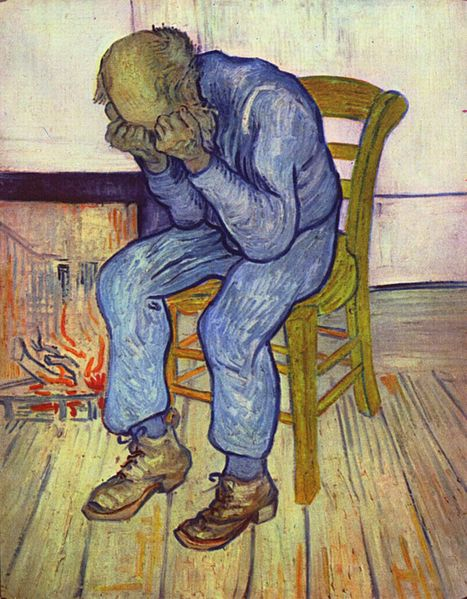
\includegraphics[width=11em]{vanGogh.jpg}}
	\end{columns}
\end{frame}
%--- Next Frame ---%

\begin{frame}[t]{Thomas Hobbes' Leviathan}
	\begin{columns}[c]
		\column{12em}
		\fbox{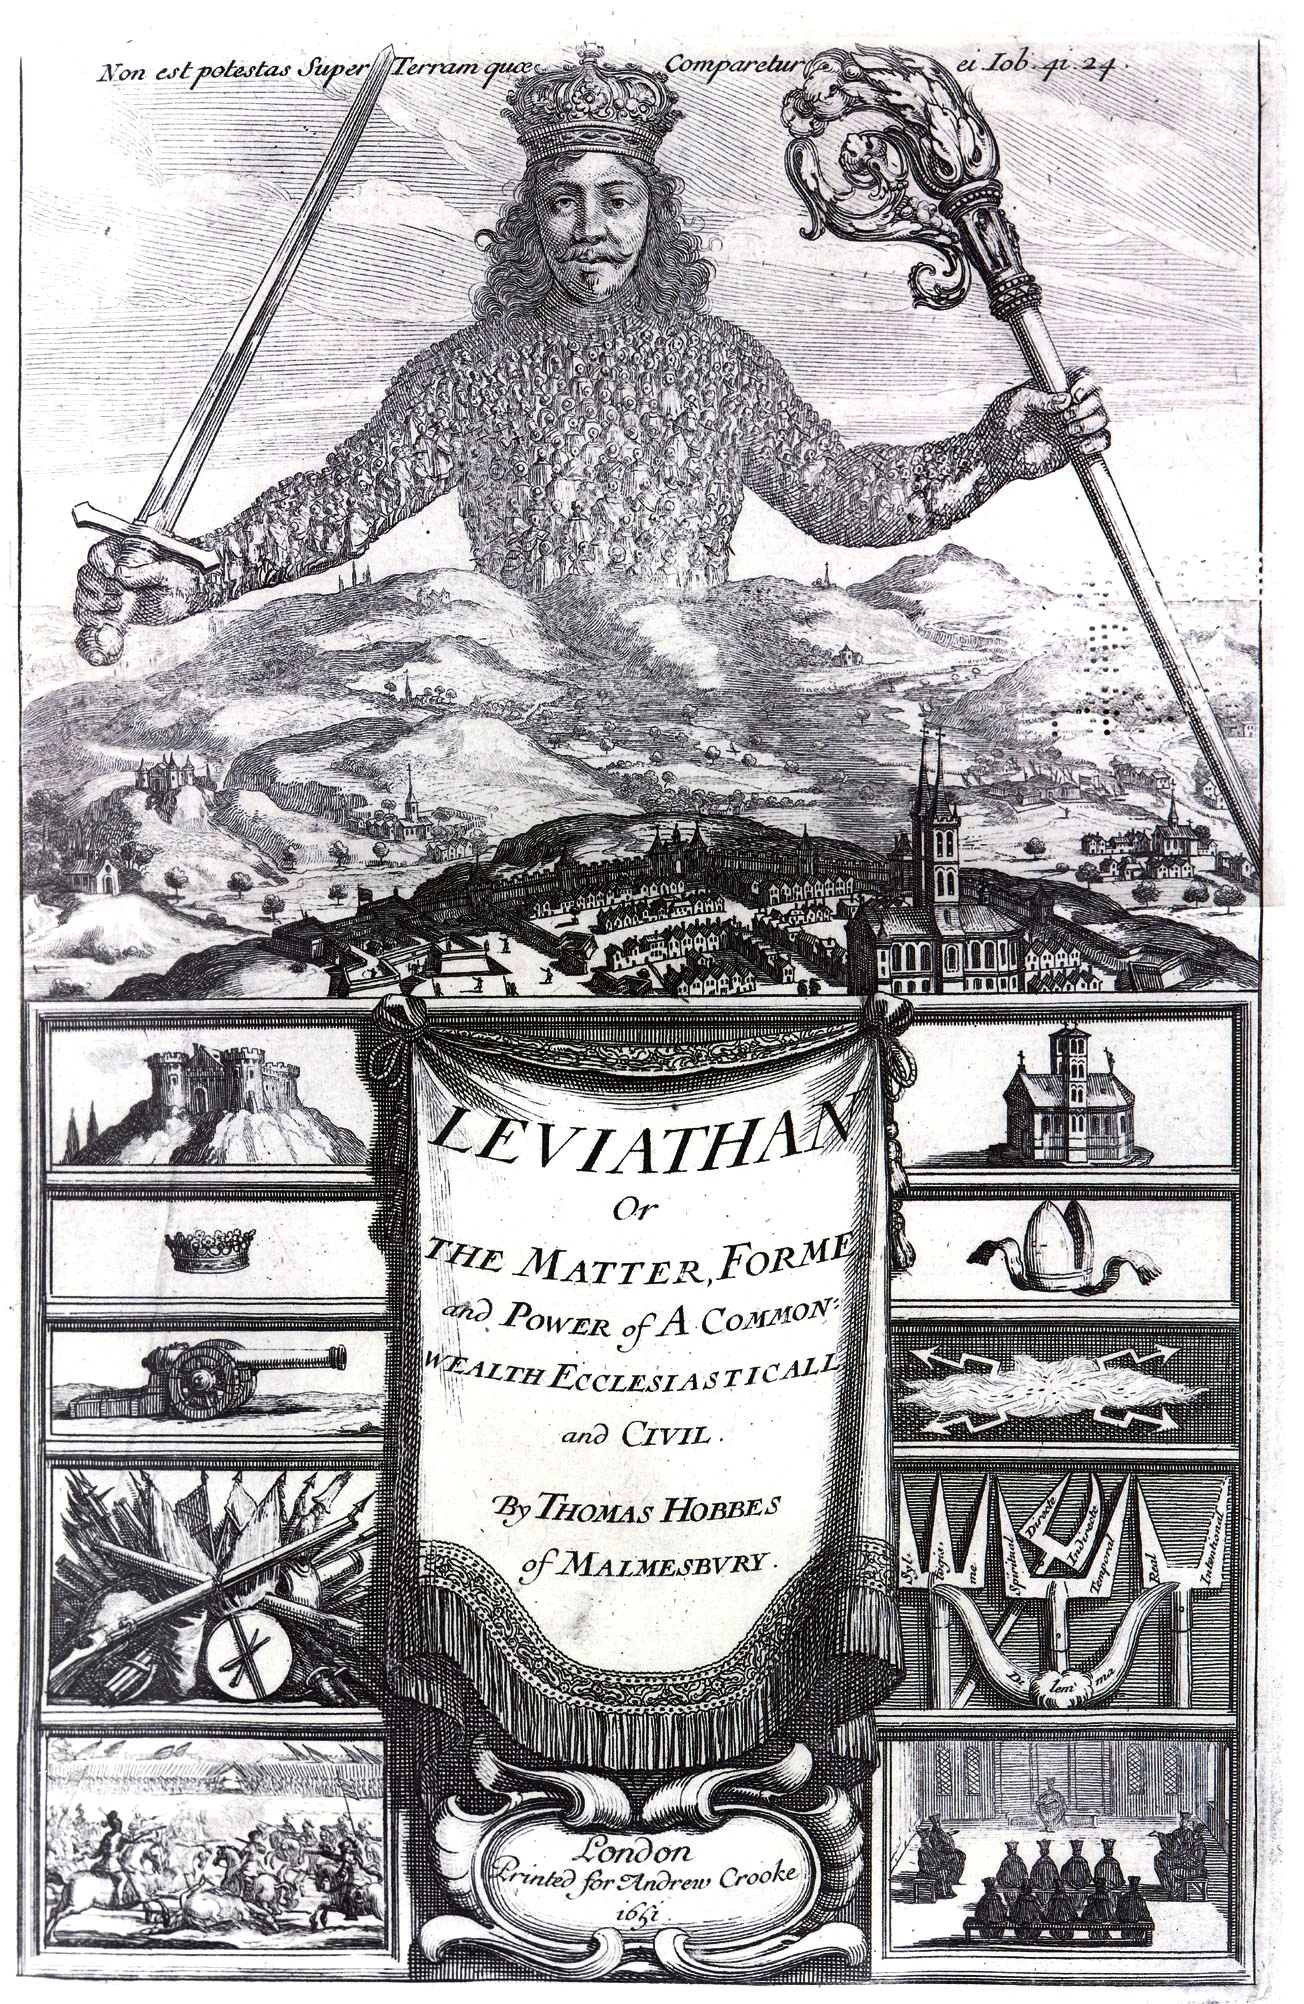
\includegraphics[width=12em]{Leviathan_gr.jpg}}
		\column{20em}
		\begin{itemize}
			\item {\itshape bellum omnium contra omnes}
			\item 죄수의 딜레마를 피하기 위해서는 사회 계약에 기반한 강력한 국가가 필요!
			\item 하지만, 이것이 전부일까? 
		\end{itemize}
	\end{columns}
\end{frame}
%--- Next Frame ---%

\begin{frame}[t]{델레마 벗어나기}
	\begin{itemize}
		\item 우리는 죄수의 딜레마를 극복할 수 있을까? 
		\item {\itshape Smith} against Hobbes?
		\item {\itshape Darwin} against Hobbes?
	\end{itemize}
\end{frame}
%--- Next Frame ---%

% section PDGame (end)

\section{게임이론의 역사} % (fold)
\label{sec:history}

\begin{frame}[t]{이론의 시작}
	\begin{columns}[c]
	\column{18em}
	\begin{itemize}
	\item 이론의 역사는 이 사람과 함께 
	\item John von Neumann (1903 -- 1957)
	\end{itemize}
	\column{14em}
	\fbox{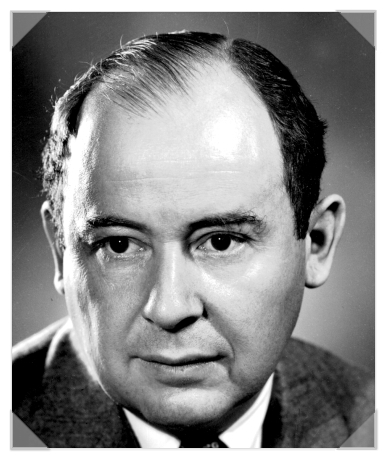
\includegraphics[width=12em]{vonNeumann.jpg}}
	\end{columns}
\end{frame}
%--- Next Frame ---%

\begin{frame}[t]{Von Neumann}
	\begin{columns}[c]
		\column{12em}
		\fbox{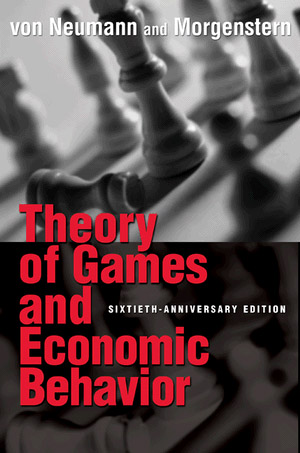
\includegraphics[width=12em]{VNM-TGEB.jpg}}
		\column{20em}
		\begin{itemize}
			\item ``Zur Theorie der Gesellschaftsspiele'' (1928) 
			\item {\itshape Theory of Games and Economic Behavior} (1944)
		\end{itemize}
	\end{columns}
\end{frame}
%--- Next Frame ---%

\begin{frame}[t]{역사적 맥락}
	\begin{columns}[c]
		\column{12em}
		\fbox{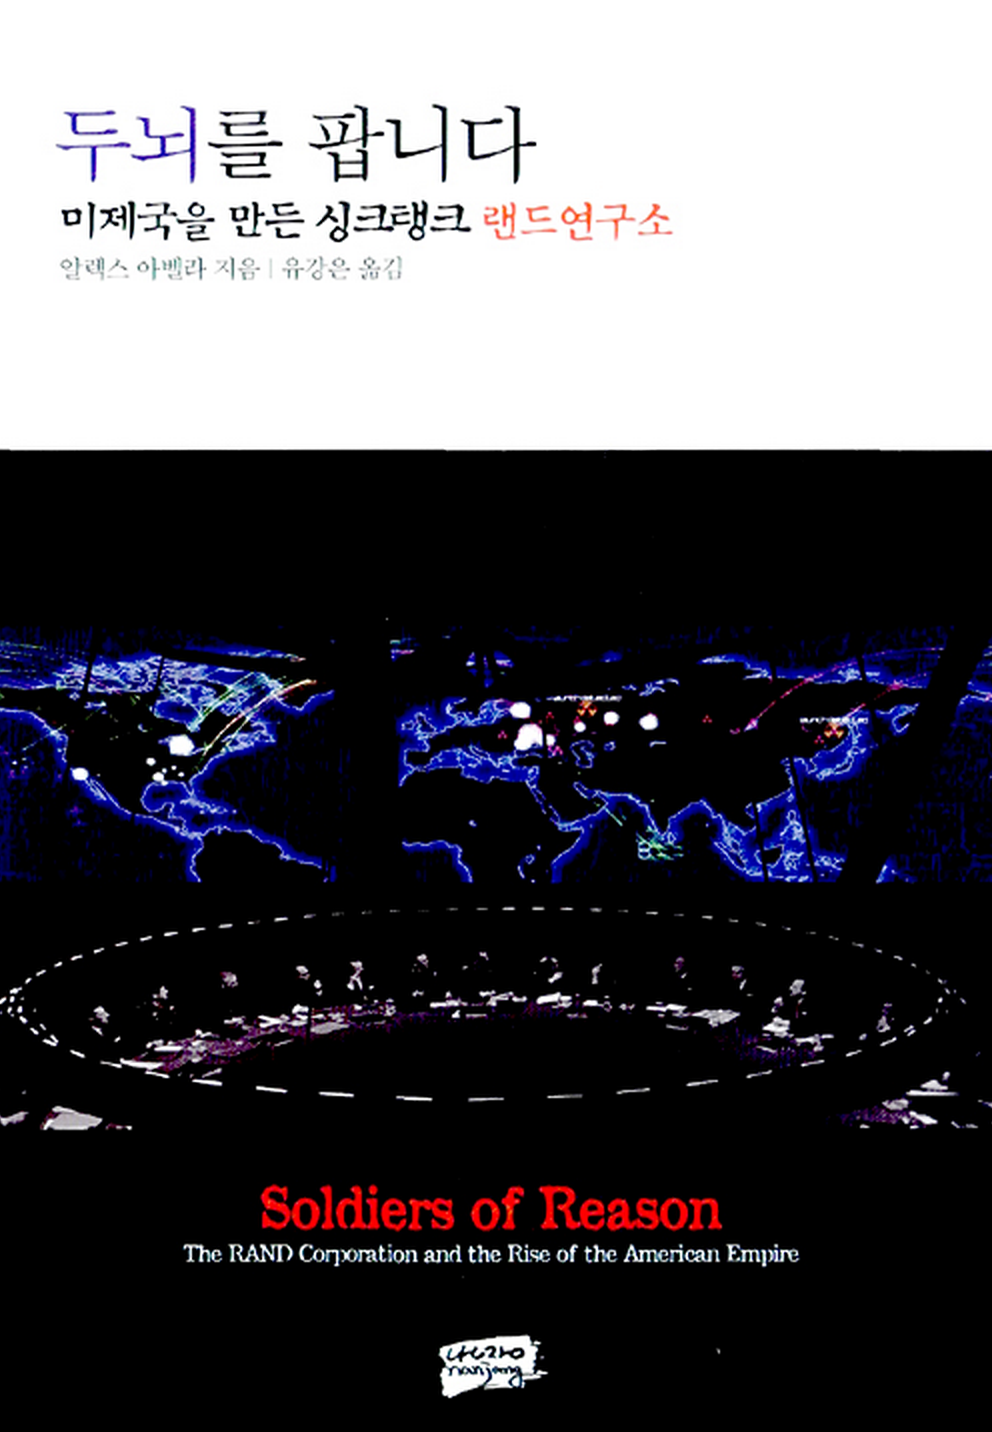
\includegraphics[width=12em]{SOR.jpg}}
		\column{20em}
		\begin{itemize}
			\item 2차 대전 이후 냉전 시대의 도래 
			\item RAND 연구소 
			\item 미국의 군사, 과학적 자원
		\end{itemize}
	\end{columns}
\end{frame}
%--- Next Frame ---%

\begin{frame}[t]{핵전쟁}
	\begin{columns}[c]
		\column{15em}
		\begin{itemize}
			\item 제로섬 게임
			\item 어떤 전략이 가장 합리적인가?  
			\item Minimax/Maxmin principle 
			\item ``mutually assured destruction''
		\end{itemize}
		\column{17em}
		\fbox{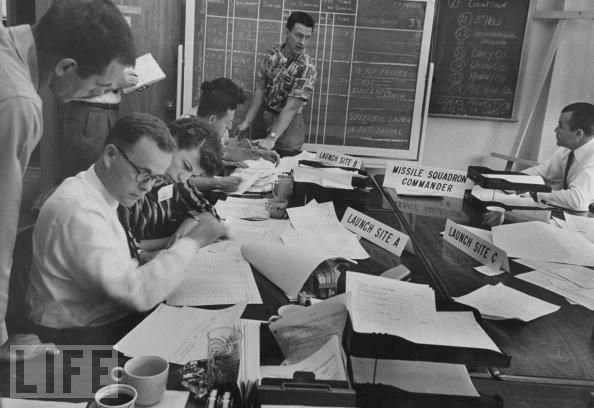
\includegraphics[width=12em]{RAND_I.jpg}}
	\end{columns}
\end{frame}
%--- Next Frame ---%

\begin{frame}[t]{Dr. Strangelove}
	\begin{columns}[c]
		\column{15em}
		\fbox{
\includegraphics[width=13em]{drstrangelove.jpg}}
		\column{15em}
		\fbox{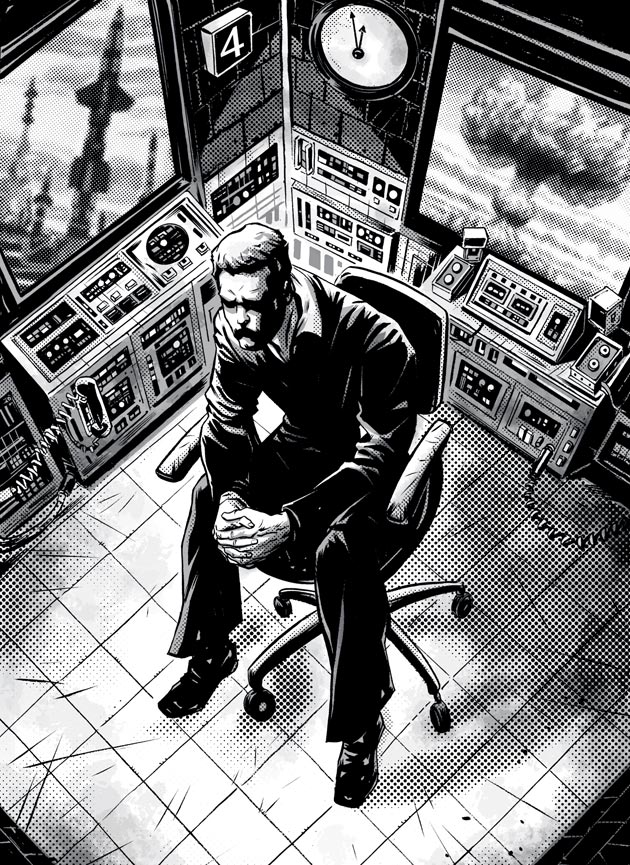
\includegraphics[width=13em]{doomsdaydevice.jpg}}
	\end{columns}
\end{frame}
%--- Next Frame ---%

\begin{frame}[t]{Beautiful Mind}
	\begin{columns}[c]
		\column{13em}
		\fbox{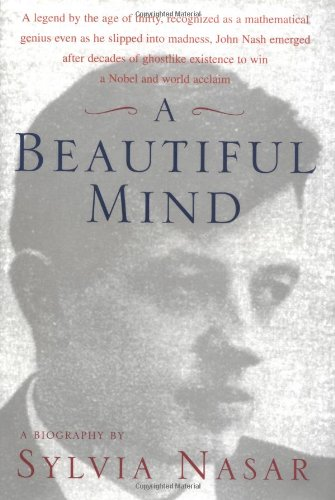
\includegraphics[width=12em]{BM_book.jpg}}
		\column{13em}
		\fbox{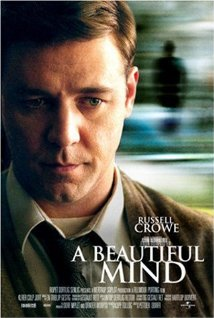
\includegraphics[width=12em]{BM_film.jpg}}
	\end{columns}
\end{frame}
%--- Next Frame ---%

\begin{frame}[t]{Nash Equilbrium}
	\begin{itemize}
		\item (어떤 종류든) 게임 일반에 ``균형''(equilibrium)이 존재할까?
		\item 그런데 균형이란 무엇일까?
		\item 내시의 수학적인 증명: \href{http://web.mit.edu/linguistics/events/iap07/Nash-Eqm.pdf}{CLICK!}
		% \item (개인적인 감상으로는) 소름끼칠 정도로 아름답다! 
		\item 게임이 연구할 만한 대상임을 세상에 보여주다. 
	\end{itemize}
\end{frame}
%--- Next Frame ---%

% section history (end)

\section{진화론과 게임이론의 만남} % (fold)
\label{sec:evoGame}

\begin{frame}[t]{진화와 게임}
	\begin{itemize}
		\item 게임이론은 초합리적인 주체를 상정 (천재들의 두뇌싸움?)
		\item 그런데, 진화는 생명체에 적용되는 보편적인 변화의 원리
		\item 지능이 없는 생명체에 어떻게 게임이론을 적용하는가? 
	\end{itemize}
\end{frame}
%--- Next Frame ---%

\begin{frame}[t]{타협과 양보}
	\begin{itemize}
	\item 게임이론에서 \\[1em]
		\begin{enumerate}
			\item 개별 행위자가 구사하는 전략과 그 어우러짐(interaction)은 남기고  
			\item 개별 행위자의 초합리성을 제거할 수 있다면 
		\end{enumerate}
	\item 진화론에서 \\[1em]
		\begin{enumerate}
			\item 개체가 자신의 이익을 추구하는 방향성으로서의 자연선택을 남기고 
			\item 이를 보다 미시적인 맥락에서 구현할 수단을 가질 수 있다면
		\end{enumerate}
	\end{itemize}
\end{frame}
%--- Next Frame ---%

\begin{frame}[t]{두 개척자}
	\begin{itemize}
		\item John Maynard Smith and George Price, ``The Logic of Animal Conflict,'' {\itshape NATURE} (1973): \href{http://www.webpages.uidaho.edu/~lukeh/giants/maynardSmith1973.pdf}{CLICK!}
		\item 진화적으로 안정적인 전략 (evolutionarily stable strategy)
		\item 게임이론의 맥락에서 진화가 처음으로 언급! 
	\end{itemize}
\end{frame}
%--- Next Frame ---%

\begin{frame}[t]{George Price}
	\begin{columns}[c]
		\column{12em}
		\fbox{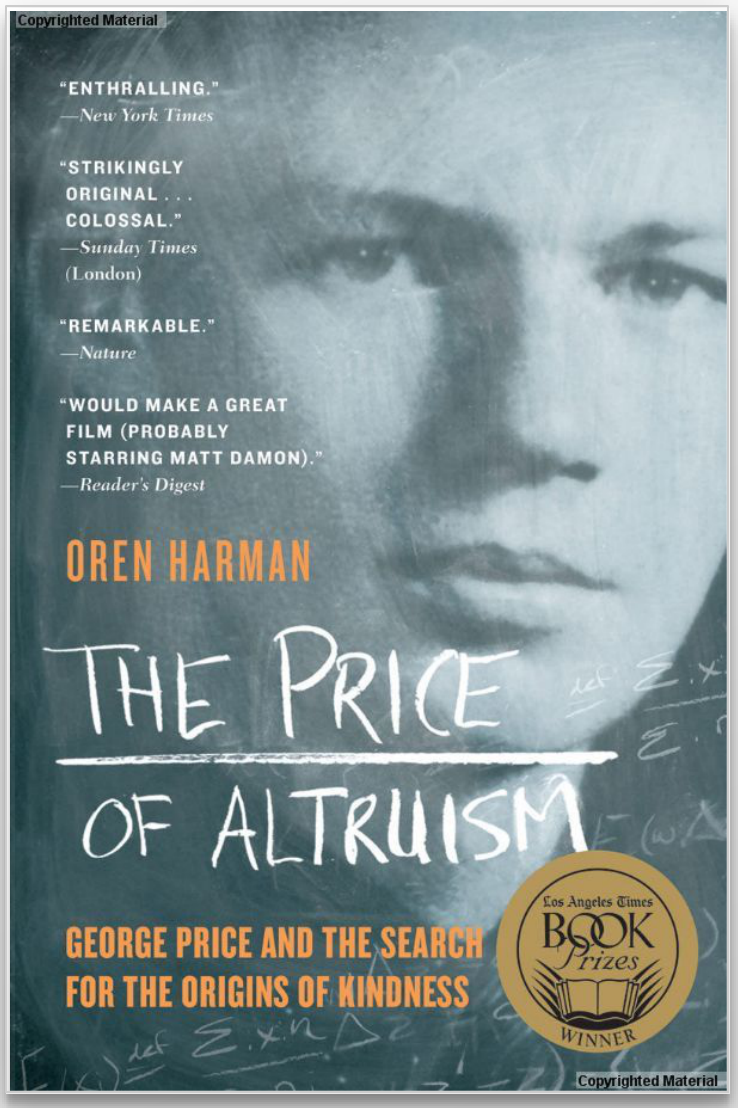
\includegraphics[width=11em]{price.png}}
		\column{18em}
		\begin{itemize}
			\item 게임이론의 진화적 응용의 실질적 창시자 
			\item Price equation 
			\item 비극적인 개인사 
		\end{itemize}
	\end{columns}
\end{frame}
%--- Next Frame ---%

\begin{frame}[t]{Hawk-Dove Game}
	\begin{columns}[c]
		\column{16em}
		\begin{itemize}
			\item 비둘기와 매의 종간 대결이 아니라! 
			\item 일단 두 마리가 벌이는 게임으로
			\item Chicken game  
		\end{itemize}
		\column{14em}
		\setlength{\tabcolsep}{0.9em}
		\begin{tabular}{|c|c|c|} \hline
			& {HAWK} &  {DOVE}\\ \hline
			{HAWK} & {\large $-\frac{1}{2}$},{\large $-\frac{1}{2}$} & {$1$}, {$0$} \\ \hline%
			 {DOVE} & $0$, $1$  & {\large $\frac{1}{2}$},{\large $\frac{1}{2}$} \\ 
			\hline
		\end{tabular}
	\end{columns}
	\pause\vspace{1em}
	\begin{columns}[c]
		\column{16em}
		\begin{itemize}
			\item 이 게임의 내시 균형은 3개!
			\item 일단, 두 개는 쉽게 찾을 수 있고... 
		\end{itemize}
		\column{14em}
		\setlength{\tabcolsep}{0.9em}
		\begin{tabular}{|c|c|c|} \hline
			& {HAWK} &  {DOVE}\\ \hline
			{HAWK} & {\large $-\frac{1}{2}$},{\large $-\frac{1}{2}$} & \color{red}{$\mathbf 1$}, \color{red}{$\mathbf 0$} \\ \hline%
			 {DOVE} & \color{red}{$\mathbf 0$}, \color{red}{$\mathbf 1$}  & {\large $\frac{1}{2}$},{\large $\frac{1}{2}$} \\ 
			\hline
		\end{tabular}
	\end{columns}
\end{frame}
%--- Next Frame ---%

\begin{frame}[t]{겁쟁이 (chicken) 게임}
	\begin{center}
		\fbox{
			\includemedia[
				width=0.7\linewidth,height=0.5\linewidth,
				activate=pageopen,
				flashvars={
					modestbranding=1 % no YT logo in control bar
					&autohide=1 % controlbar autohide
					&showinfo=0 % no title and other info before start
					&rel=0 % no related videos after end
				}
			]{}{http://www.youtube.com/v/u7hZ9jKrwvo}
		}
	\end{center}
\end{frame}
%--- Next Frame ---%

\begin{frame}[t]{혼합 전략 (Mixed Strategy)}
	\begin{columns}[c]
		\column{16em}
		\begin{itemize}
			\item Hawk를 $p$의 확률로 Dove를 $1-p$의 확률로 
			\item 균형은 나의 '기대 보수'를 극대화해주는 $p$
		\end{itemize}
		\column{14em}
		\setlength{\tabcolsep}{0.9em}
		\begin{tabular}{|c|c|c|} \hline
			& {HAWK} &  {DOVE}\\ \hline
			{HAWK} & {\large $-\frac{1}{2}$},{\large $-\frac{1}{2}$} & {$1$}, {$0$} \\ \hline%
			 {DOVE} & $0$, $1$  &  {\large $\frac{1}{2}$},{\large $\frac{1}{2}$}  \\ 
			\hline
		\end{tabular}
	\end{columns}
	\begin{itemize}
		\item 이 게임의 혼합 균형은 HAWK를 $1/2$의 확률로 구사하는 것
		\item 이 `혼합' 균형만이 진화적으로 안정적이다! 
	\end{itemize}
\end{frame}
%--- Next Frame ---%

\begin{frame}[t]{학습 (learning)}
	\begin{itemize}
		\item 플레이어는 전략을 타고 난다.\\[1em]
		\begin{enumerate} 
			\item 해당 전략이 좋다면, 계속 고수 ({\color{gray}{혹은 더 많은 자손}}) 
			\item 해당 전략이 나쁘다면, 다른 전략으로 수정 ({\color{gray}{혹은 더 적은 자손}})
		\end{enumerate}
			\item 초합리성에서 더 나은 것을 향한 `학습'으로 
			\item 정태 (statics)에서 동태(dynamics)로
	\end{itemize}
\end{frame}
%--- Next Frame ---%

\begin{frame}[t]{진화적 관점만으로는..}
	\begin{itemize}
		\item 죄수의 딜레마는 해결할 수 없다! \\(대단히 표준적인 가정 아래 있다면...)
	\end{itemize}
	\begin{center}
		\fbox{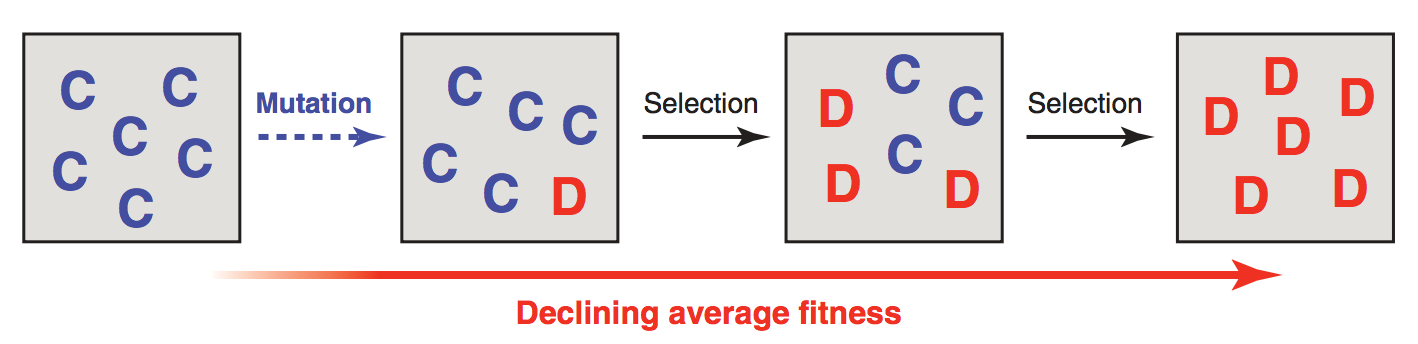
\includegraphics[width=30em]{decline.png}}
	\end{center}
\end{frame}
%--- Next Frame ---%

% section evoGame (end)

\section{협력으로 가는 5가지 길} % (fold)
\label{sec:cooperation}

\begin{frame}[t]{지금까지의 요약}
	\begin{columns}[c]
		\column{15em}
		\begin{itemize}
			\item 인간이 이익을 추구하고 
			\item 서로간의 이익이 상충할 때 
			\item 세상의 모습은...
		\end{itemize}
		\column{20em}
			\fbox{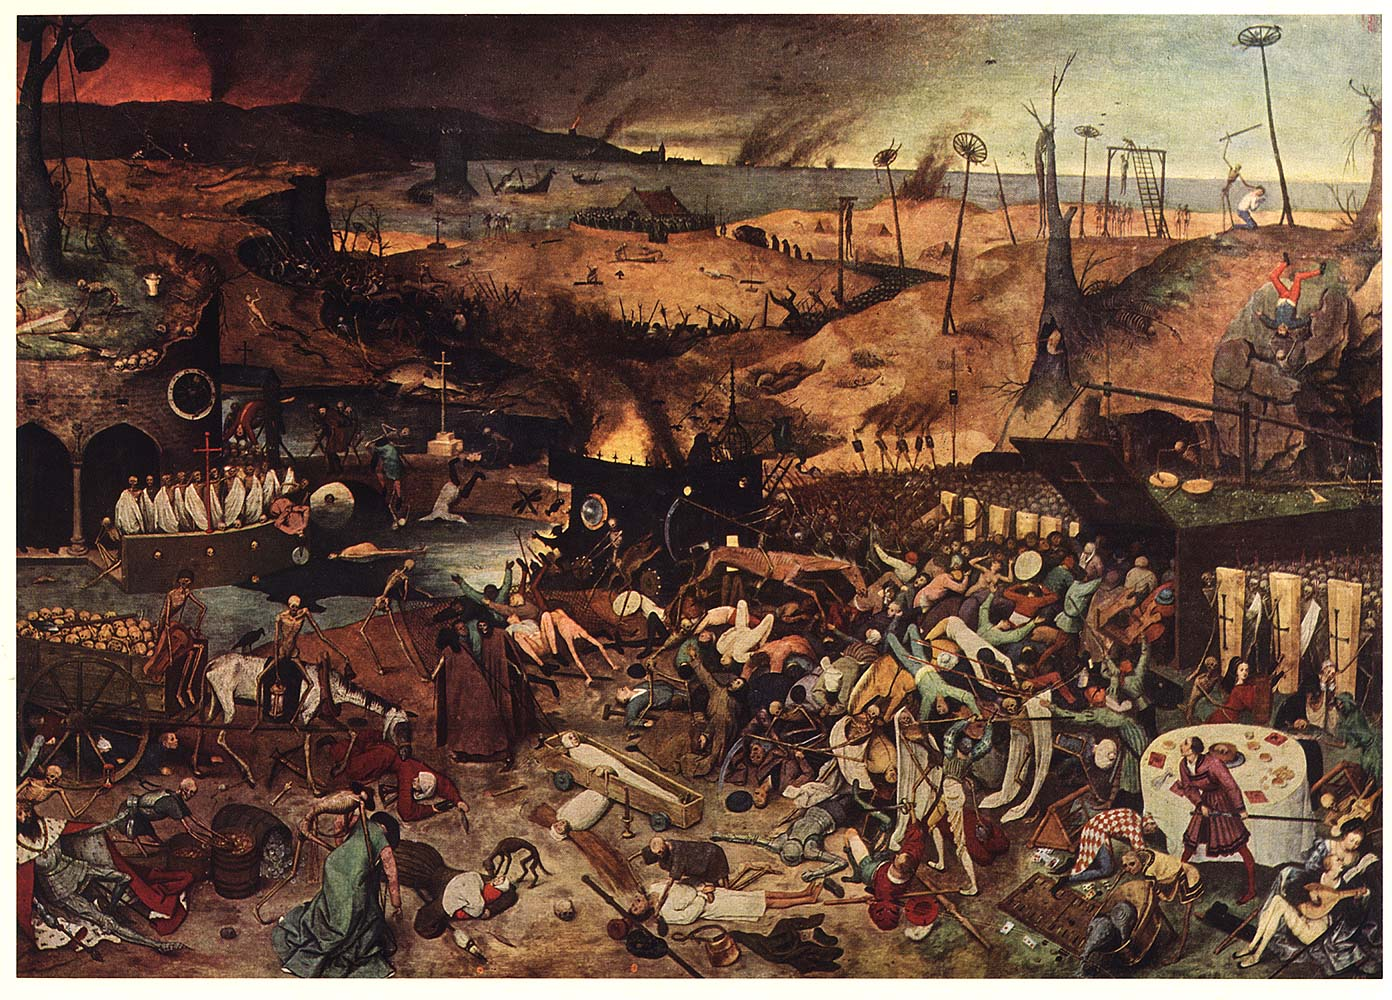
\includegraphics[width=18em]{brueghel.jpg}}
	\end{columns}
\end{frame}
%--- Next Frame ---%

\begin{frame}[t]{PD 보수행렬}
	\begin{columns}[c]
		\column{15em}
		\begin{itemize}
			\item 대표적으로 쓰이는 보수행렬
			\item 두 명이 대칭적이므로 한 명의 보수만 쓰자.
			\item $b$: 이득(benefit), $c$: 비용(cost) 
			\item 딜레마가 되려면? $b>c$
		\end{itemize}
		\column{20em}
		\begin{table}
			\setlength{\tabcolsep}{1.2em}
			\begin{tabular}{|c|c|c|} \hline
				& {C} &  {D}\\ \hline
				{C} & {$b-c$} & {$-c$} \\ \hline%
				{D} & {$b$}    & {$0$} \\ 
				\hline
			\end{tabular}
		\end{table}
	\end{columns}
\end{frame}
%--- Next Frame ---%

\begin{frame}[t]{왜 진화인가?}
	\begin{columns}[c]
		\column{13em}
		\fbox{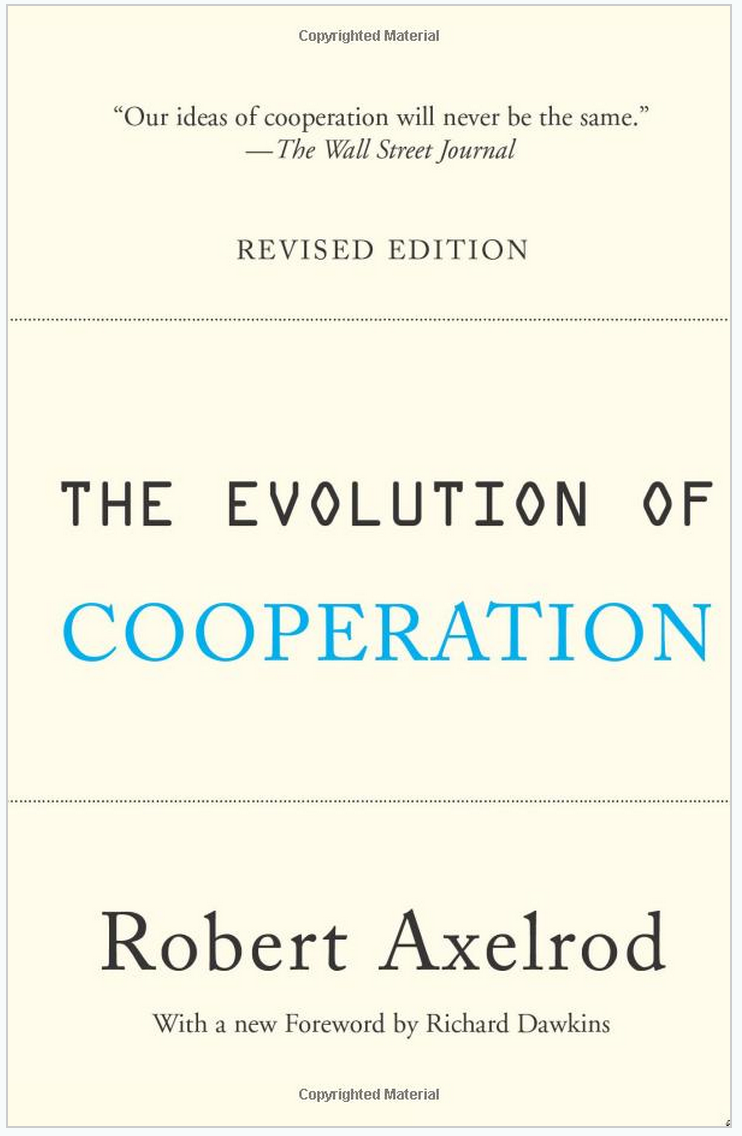
\includegraphics[width=11em]{axelrod.png}}
		\column{18em}
		\begin{itemize}
			\item 권위(국가)를 통한 해결은 완전하지도 바람직하지도 않다. 
			\item 왜 '진화'인가? 
			\item 혹은 딜레마는 어떻게 '변형'되는가? 
		\end{itemize}
	\end{columns}
\end{frame}
%--- Next Frame ---%

\begin{frame}[t]{Martin Nowak}
	\begin{columns}[c]
		\column{20em}
		\begin{itemize}
			\item 협력의 진화를 터준 5가지 경로 혹은 변형\\(물론, 유일하거나 절대적인 것은 아니야!)
			\item 게임이론을 통한 통일적 접근 
			\item 협력에 관한 최신의 (쉽고?) 수학적인 지도의 완성
		\end{itemize}
		\column{12em}
		\fbox{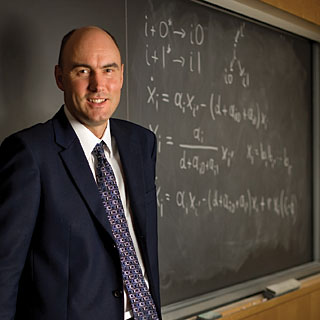
\includegraphics[width=10em]{nowak_2.jpg}}
	\end{columns}
\end{frame}
%--- Next Frame ---%

\begin{frame}[t]{한 눈에 보는 5가지 길 (1)}
	\begin{columns}[c]
		\column{10em}
		\fbox{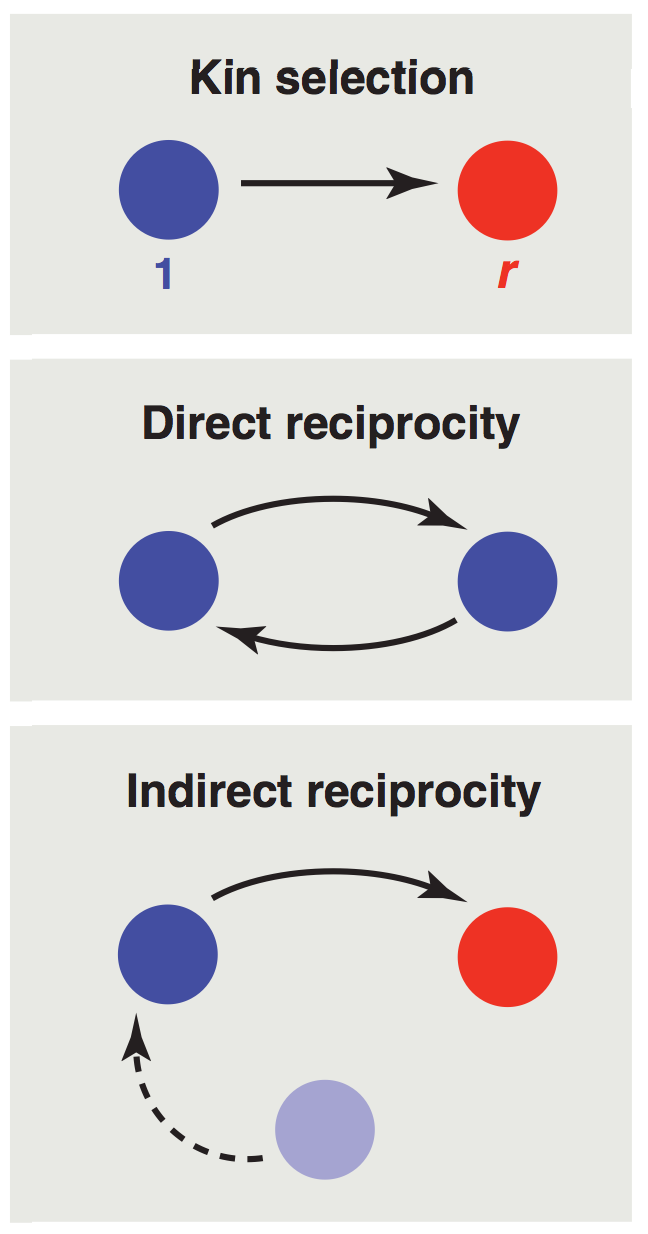
\includegraphics[width=10em]{five_1.png}}
		\column{20em}
		\vspace{-1em}
		\begin{itemize}
			\item ``네 이익이 나의 이익과 같다면'' \\[4em]
			\item ``네가 나를 돕는다면''\\[5em]
			\item ``그이가 저이를 도왔기에'' 
		\end{itemize}
	\end{columns}
\end{frame}
%--- Next Frame ---%

\begin{frame}[t]{한 눈에 보는 5가지 길 (2)}
	\begin{columns}[c]
		\column{10em}
		\fbox{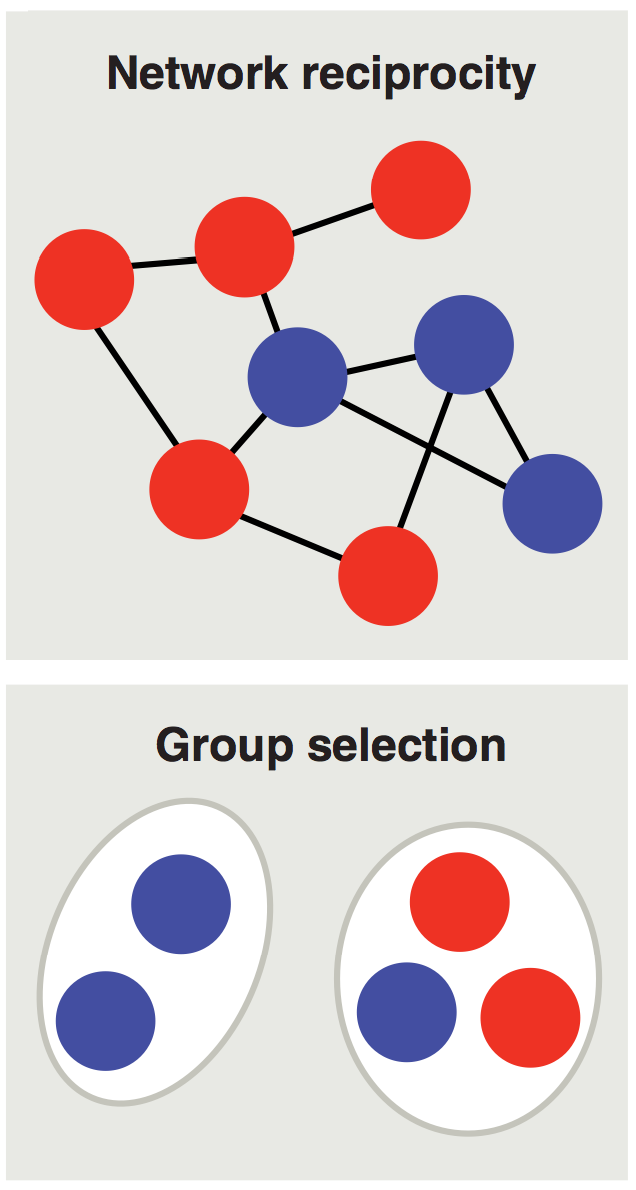
\includegraphics[width=10em]{five_2.png}}
		\column{20em}
		\vspace{0em}
		\begin{itemize}
			\item ``그들이 나와 같다면'' \\[8em]
			\item ``우리가 그들을 물리칠 수 있다면''
		\end{itemize}
	\end{columns}
\end{frame}
%--- Next Frame ---%

\begin{frame}[t]{다섯 가지 길을 한마디로 한다면}
	\begin{columns}[c]
		\column{12em}
		\begin{itemize}
			\item PD 게임의 변형! 
			\item 다른 게임으로 바뀌면, 딜레마가 극복될 가능성이 제시
			\item 혼돈의 야수를 길들이는 방법
		\end{itemize}
		\column{18em}
		\fbox{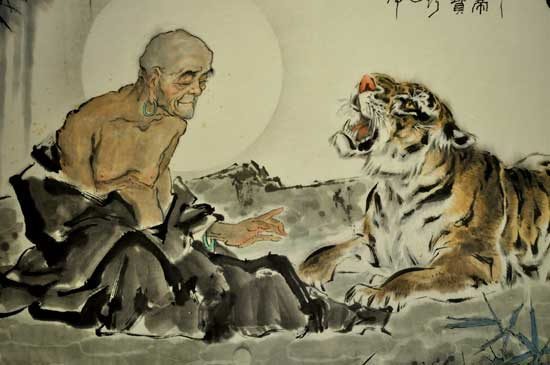
\includegraphics[width=17em]{tiger.jpg}}
	\end{columns}
\end{frame}
%--- Next Frame ---%

\begin{frame}[t]{집단선택 (group selection)}
	\begin{columns}[c]
		\column{12em}
		\begin{itemize}
			\item 집단간의 대립이 필수
			\item 이에 방해가 된다면?
			\item 동조화, 획일화 경향
		\end{itemize}
		\column{18em}
		\fbox{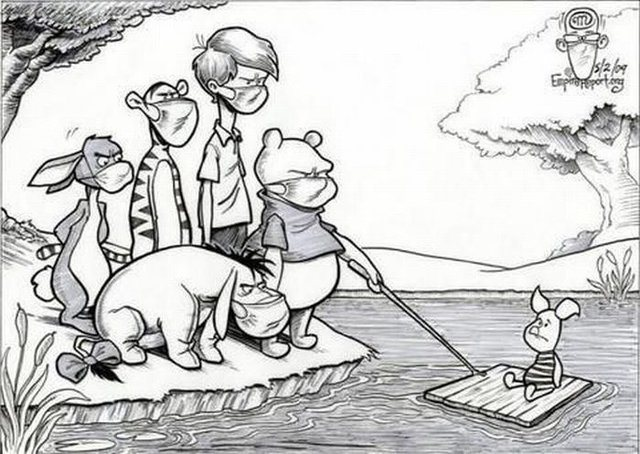
\includegraphics[width=17em]{ostracism.jpg}}
	\end{columns}
\end{frame}
%--- Next Frame ---%

\begin{frame}[t]{초협력자를 향하여}
	\begin{columns}[c]
		\column{12em}
		\begin{itemize}
			\item 인간 협력의 현단계는 가족, 출신, 국가, 민족에 포획 
			\item 또다른 단계로의 진화를 요구하는 압박 
			\item 초협력자란?
		\end{itemize}
		\column{18em}
		\fbox{
\includegraphics[width=17em]{ubuntu.png}}
	\end{columns}
\end{frame}
%--- Next Frame ---%

\begin{frame}[t]{간단한 행동실험: Guessing Game}
	\begin{itemize}
		\item 칠판에 그은 선의 길이를 맞춰보자. 
		\item 실제 길이에 가장 근접하게 맞추는 학생(들)에게 문화상품권 (5000) 증정
	\end{itemize}
\end{frame}
%--- Next Frame ---%

% section cooperation (end)


\end{document}